\section{Experimental Results}\label{sec:results}
For initial evaluation of FSMDriver, only changes in the transition function's 
parameters were tested, with a simple iteration over arbitrary values for all. At
each iteration, only one parameter value was changed. Table \ref{tbl:parameters} shows the parameters, their initial ($V_I$) and final 
($V_F$) values, and the step ($\Delta$) taken in each iteration. 

\begin{table}[h]
\renewcommand{\arraystretch}{1.3}
\caption{Transition Parameters}
\label{tbl:parameters}
\centering
\begin{tabular}{c||c||c||c}
\hline \bfseries &\bfseries $V_I$ &\bfseries $V_F$ &\bfseries $\Delta$ \\
\hline
\hline MSD & $20$ & $200$ & $5$ \\ 
\hline LE & $-1$ & $-0.8$ & $0.1$ \\ 
\hline RE & $0.8$ & $1$ & $0.1$ \\ 
\hline ST & $30$ & $300$ & $10$ \\ 
\hline 
\end{tabular} 
\end{table}

For each of the over 8500 configurations, experiments consisted of 3 laps, in 
the B-Speedway and CG-Speedway 1 tracks (see Fig. \ref{fig:tracks}), each race 
starting with one car fully stopped. B-Speedway provides the simplest track for 
validation, while CG-Speedway 1 has more characteristics of usual race tracks, 
such as sharp curves for either side, and provides a more general idea of the 
FSMDriver's behavior.

\begin{figure}
\centering 
\subfloat[B-Speedway]{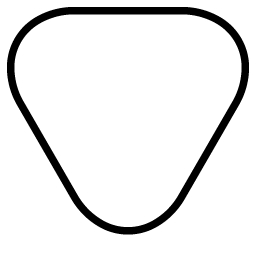
\includegraphics[width=1.2in]{B-Speedway}}
% \label{fig_first_case}} 
\hfill
\subfloat[CG-Speedway]{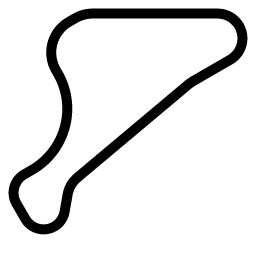
\includegraphics[width=1.2in]{CG-Speedway}}
% \label{fig_second_case}} 
\caption{FSMDriver test tracks.} 
\label{fig:tracks} 
\end{figure} 

Results are evaluated by total race time, smaller being better. The parameter values 
for the fastest races are presented in Table \ref{tbl:best_config}.
It is interesting to note that many configurations yielded the same results, and 
that \textbf{Straigh Line}'s steering control is sufficient for it to run on wide
curves, there no transitions were triggered in B-Speedway's tests.

\begin{table}[h]
% \renewcommand{\arraystretch}{1.3}
\caption{Best Configuration}
\label{tbl:best_config}
\centering
\begin{tabular}{c||c||c||c||c}
\hline & MSD & LE & RE & ST \\ \hline\hline
B-Speedway & 20 & -0.8 & 1 & 110 \\\hline
CG-Speedway 1 & 20 & -0.8 & 1 & 110 \\\hline
\end{tabular} 
\end{table}

To further analyze FSMDriver's behavior, it is  
compared to default controllers provided by the TORCS distribution. One of the 
maintainers of TORCS, Bernhard Wymann\footnote{www.berniw.org}, has created
a wide range of controllers with diverse characteristics, from average racing 
behavior like \emph{berniw3} to one of the best controllers available \emph{berniw1}.
In this test, controllers had a 3 lap race (by themselves) and total time was 
evaluated. Results are shown in Tables \ref{tbl:berniw_B} and \ref{tbl:berniw_CG}.

\begin{table}[h]
\renewcommand{\arraystretch}{1.3}
\caption{3 Laps in B-Speedway}
\label{tbl:berniw_B}
\centering
\begin{tabular}{c||c||c||c}
\hline
\bfseries Driver & \bfseries Total Time & \bfseries Damage & \bfseries Top Speed \\ 
\hline
\hline Berniw 1 & 02:25:65 & 6 & 321 \\
\hline Berniw 2 & 02:25:65 & 6 & 321 \\
\hline Berniw 7 & 02:27:20 & 0 & 308 \\
\hline Berniw 6 & 02:27:46 & 0 & 309 \\
\hline Berniw 8 & 02:27:75 & 0 & 307 \\
\hline Berniw 9 & 02:28:10 & 0 & 306 \\
\hline Berniw 5 & 02:28:58 & 2 & 307 \\
\hline Berniw 4 & 02:29:42 & 3 & 303 \\
\hline Berniw 3 & 02:31:38 & 0 & 301 \\
\hline FSMDriver & 02:34:95 & 1 & 299 \\ 
\hline Berniw 10 & 02:40:70 & 8 & 282 \\ 
\hline 
\end{tabular}
\end{table}

\begin{table}[h]
\renewcommand{\arraystretch}{1.3}
\caption{ 3 Laps in CG Speedway 1}
\label{tbl:berniw_CG}
\centering

\begin{tabular}{c||c||c||c}
\hline \bfseries Driver &\bfseries Total Time &\bfseries Damage &\bfseries Top Speed \\
\hline
\hline Berniw 8 & 02:07:17 & 0 & 246 \\
\hline Berniw 6 & 02:07:18 & 0 & 248 \\
\hline Berniw 4 & 02:07:18 & 0 & 246 \\
\hline Berniw 7 & 02:07:20 & 0 & 250 \\
\hline Berniw 5 & 02:07:28 & 0 & 246 \\
\hline Berniw 3 & 02:07:28 & 0 & 247 \\
\hline Berniw 9 & 02:07:58 & 0 & 247 \\
\hline Berniw 1 & 02:12:80 & 1 & 252 \\
\hline Berniw 2 & 02:12:80 & 1 & 252 \\
\hline Berniw 10 & 02:21:54 & 0 & 230 \\
\hline FSMDriver & 02:34:49 & 3337 & 242 \\ 
\hline 
\end{tabular}
\end{table}

As expected, this initial version of FSMDriver does not have the outstanding 
behavior of \emph{berniw1}, but its results show that the proposal does have
acceptable performance, and future tweaking of FSMDriver's states parameters may
lead to better results. It is also important to note that the TORCS controllers
have a different implementation, one that has access to the simulator's inner data,
while FSMDriver's behavior is defined exclusively by its available sensors.

After analyzing FSMDriver's performance in CG-Speedway 1, it was clear from the
amount of damage that the problem was that the controller was consistently going
out of the track and hitting the wall. After further inspection, this was found 
to happen after stretches of straight lines, when FSMDriver would accelerate as 
much as possible and enter a curve going too fast for proper steering.

This indicates the need for another state, \textbf{Approaching Curve}, in which 
FSMDriver would adjust between current behaviors and enter the curve in a better
condition to make it as fast as possible.